\documentclass{beamer}
\usepackage{FiraSans}
\usetheme{metropolis}           % Use metropolis theme
\usepackage{xgreek}
\title{Automated Data Scientist}
\date{Δεκέμβριος, 2016}
\author{Νησιώτη Ελένη \\AEM : 7737 \\ Επιβλέπων: Χατζηδημητρίου Κυριάκος}
\institute{Αριστοτέλειο Πανεπιστήμιο Θεσσαλονικής \\ ΗΜΜΥ}
\setlength{\parskip}{\baselineskip}%
\usepackage{graphicx}
\graphicspath{{./images/}}
\usepackage[backend=biber]{biblatex}
\addbibresource{bibliography.bib}
\usepackage{fontspec}
\setmainfont[Ligatures=TeX]{Linux Libertine O}
\begin{document}
  \maketitle
  \section{Σκοπός διπλωματικής εργασίας}
  \begin{frame}{ \scshape Το πρόβλημα}
   To $ 75 \% $ ενός πειράματος μηχανικής μάθησης αφιερώνεται στην προετοιμασία της εφαρμογής του αλγορίθμου και το $15 \% $ στα βήματα που την ακολουθούν. Το μεγαλύτερο μέρος της έρευνας επικεντρώνεται στο ενδιάμεσο $10 \%$ ...
   \\[12pt]
   \rightline{{\rm --- Rich Caruana}}
   \rightline{{\rm Automl 2016 $@$ ICML}}
  \end{frame}
  
  \begin{frame}{ \scshape Η επιστήμη του Automl}
  	\begin{minipage}[t]{.4\textwidth}  		
  		Απαρχές
  		\vspace{4ex}
  	\end{minipage}% This must go next to `\end{minipage}` \hspace{2cm}
  	  	\begin{minipage}[t]{.5\textwidth}
  	  		Unica, MarketSwitch, KXEN  	
  	  		\vspace{4ex}
  	  	\end{minipage}
  	\begin{minipage}[t]{.4\textwidth}  		
  		Πεδία Εφαρμογής
  		\vspace{4ex}
  	\end{minipage}% This must go next to `\end{minipage}` \hspace{2cm}
  	\begin{minipage}[t]{.5\textwidth}
  		Προεπεξεργασία, Ρύθμιση αλγορίθμου, Αξιολόγηση και κατανόηση μοντέλου
  		\vspace{4ex} 
  	\end{minipage}
  	\begin{minipage}[t]{.4\textwidth}  		
  		Σύγχρονα Εργαλεία
  		\vspace{4ex}
  	\end{minipage}% This must go next to `\end{minipage}` \hspace{2cm}
	\begin{minipage}[t]{.5\textwidth}
  		AutoWeka, Microsoft Azure, caret, HPOlib
  		\vspace{4ex}
  	\end{minipage}
  \end{frame}
  
  \begin{frame} { \scshape Προτεινόμενο σύστημα}
  	Ένας \alert{αυτοματοποιημένος} αναλυτής δεδομένων για προβλήματα δυαδικής ταξινόμησης με \alert{εμπειρία} παλαιότερων πειραμάτων και \alert{κατανοητή} έξοδο.
  	
  \end{frame}
  
  \begin{frame} { \scshape Γνώσεις που αποκτήθηκαν}
  	R
  	
  	Automl
  	
  	Τεχνολογία Λογισμικού
  	
  \end{frame}
  \section{Μεθοδολογία}
  \begin{frame} { \scshape Ρύθμιση αλγορίθμου μηχανικής μάθησης}
  	\begin{minipage}[t]{.3\textwidth}  		
  		Σκοπός
  		\vspace{4ex}
  	\end{minipage}% This must go next to `\end{minipage}` \hspace{2cm}
  	\begin{minipage}[t]{.6\textwidth}
  		Βελτιστοποίηση υπερπαραμέτρων αλγορίθμου  	
  		\vspace{4ex}
  	\end{minipage}
  	\begin{minipage}[t]{.3\textwidth}  		
  		Τεχνική
  		\vspace{4ex}
  	\end{minipage}% This must go next to `\end{minipage}` \hspace{2cm}
  	\begin{minipage}[t]{.6\textwidth}
  		Bayesian βελτιστοποίηση
  		\vspace{4ex} 
  	\end{minipage}
  	\begin{minipage}[t]{.3\textwidth}  		
  		Ιδέα
  		\vspace{4ex}
  	\end{minipage}% This must go next to `\end{minipage}` \hspace{2cm}
  	\begin{minipage}[t]{.6\textwidth}
  		Αντικατάσταση της χρονοβόρας διαδικασίας βελτιστοποίησης με πρόβλεψη
  		\vspace{4ex}
  	\end{minipage}
  	\begin{minipage}[t]{.3\textwidth}  		
  		Υλοποίηση
  		\vspace{4ex}
  	\end{minipage}% This must go next to `\end{minipage}` \hspace{2cm}
  	\begin{minipage}[t]{.6\textwidth}
  		Εισαγωγή μετα-μάθησης για παραγωγή χαρακτηριστικών χρήσιμων σε ένα νευρωνικό πρόβλεψης των βέλτιστων υπερπαραμέτρων (HPPNN).
  		\vspace{4ex}
  	\end{minipage}
  \end{frame}
  \begin{frame}{ \scshape Bayesian Βελτιστοποίηση}
  	\begin{minipage}[t]{0.7\textwidth}
  	\begin{figure}
  		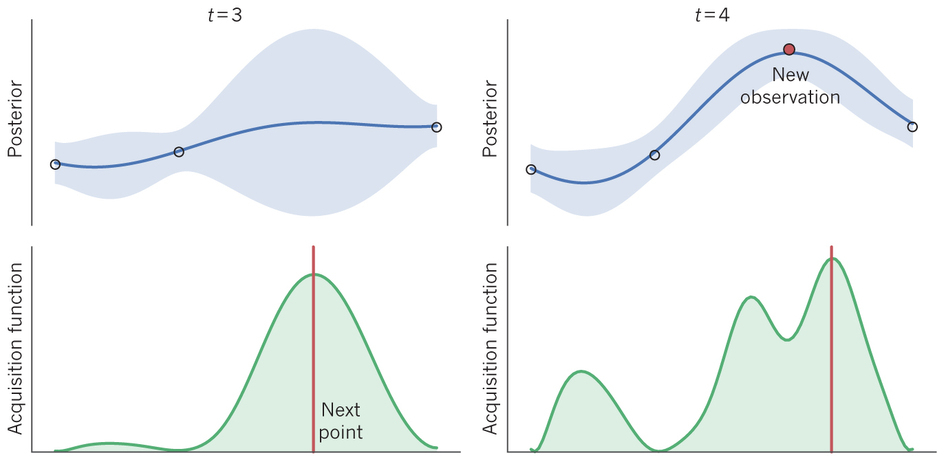
\includegraphics[width=\textwidth]{bayes}
  		\caption{Μία γενιά Bayesian Βελτιστοποίησης με Γκαουσιανές διαδικασίες}
  	\end{figure}
  \end{minipage} \hspace{0.5cm}
  	\begin{minipage}[t]{0.2\textwidth}
  		\centering
  		TPE
  		\\ \vspace{1cm}
  		Spearmint
  		\\ \vspace{1cm}
  		SMAC
  	\end{minipage}
  \end{frame}
  \begin{frame}{ \scshape Μετα-μάθηση}
  	\begin{minipage}[t]{.3\textwidth}  		
  		Σκοπός
  		\vspace{4ex}
  	\end{minipage}% This must go next to `\end{minipage}` \hspace{2cm}
  	\begin{minipage}[t]{.6\textwidth}
  		Δημιουργία μετα-γνώσης από πειράματα μηχανικής μάθησης  	
  		\vspace{4ex}
  	\end{minipage}
  	\begin{minipage}[t]{.3\textwidth}  		
  		Τρόπος
  		\vspace{4ex}
  	\end{minipage}% This must go next to `\end{minipage}` \hspace{2cm}
  	\begin{minipage}[t]{.6\textwidth}
  		Εξαγωγή μετα-χαρακτηριστικών των σετ δεδομένων, τα οποία περιέχουν ουσιώδη πληροφορία
  		\vspace{4ex} 
  	\end{minipage}
  	\begin{minipage}[t]{.3\textwidth}  		
  		Εφαρμογές
  		\vspace{4ex}
  	\end{minipage}% This must go next to `\end{minipage}` \hspace{2cm}
  	\begin{minipage}[t]{.6\textwidth}
  		Αρχικοποίηση αλγορίθμων βελτιστοποίησης
  		\vspace{4ex}
  	\end{minipage}
  \end{frame}
  \begin{frame}{ \scshape Bάση ευριστικών}
  	
  \end{frame}
   \begin{frame}{ \scshape Ensemble forward selection}
   	[]
   \end{frame}
   \section{Αρχιτεκτονική Συστήματος}
   \begin{frame}{ \scshape Υποσύστημα εκπαίδευσης}
   	\begin{figure}
   		\includegraphics[width=\textwidth]{train}
   		\caption{Θα αλλαχθεί, το βάζω για αναφορά}
   	\end{figure}
   \end{frame}
   \begin{frame}{ \scshape Υποσύστημα πρόβλεψης}
   	\begin{figure}
   		\includegraphics[width=\textwidth]{predict}
   		\caption{Θα αλλαχθεί, το βάζω για αναφορά}
   	\end{figure}
   \end{frame}
   \section{Πειραματικά Αποτελέσματα}
  \begin{frame}{ \scshape Περιγραφή πειραμάτων}
  	\begin{minipage}[t]{.3\textwidth}  		
  		Σετ δεδομένων
  		\vspace{4ex}
  	\end{minipage}% This must go next to `\end{minipage}` \hspace{2cm}
  	\begin{minipage}[t]{.6\textwidth}
  		50 σετ δυαδικής ταξινόμησης από το UCI Repository.
  		  	
  		\vspace{4ex}
  	\end{minipage}
  	\begin{minipage}[t]{.3\textwidth}  		
  		Off-line
  		\vspace{4ex}
  	\end{minipage}% This must go next to `\end{minipage}` \hspace{2cm}
  	\begin{minipage}[t]{.6\textwidth}
  		Βελτιστοποίηση των αλγορίθμων SVM, NN, Tree, Bayes της caret με χρήση της βιβλιοθήκης HPOlib με hold-out validation, εξαγωγή μετα-χαρακτηριστικών και εκπαίδευση νευρωνικού με 10-fold CV.
  		
  		
  		[Χρόνος και hardware]
  		\vspace{4ex} 
  	\end{minipage} 
  \end{frame}
  \begin{frame}{ \scshape Αξιολόγηση HPPNN} 
  	[διαγράμματα]
  \end{frame}
  \begin{frame}{ \scshape Αξιολόγηση συστήματος} 
  	[διαγράμματα]
  \end{frame}
  \begin{frame}{ \scshape Συμπεράσματα} 
  	Η επιστήμη του automl επιδιώκει ένα συμβιβασμό μεταξύ αυτοματοποίησης και κατανοησιμότητας (intuition). Το λογισμικό που σχεδιάσαμε συνδυάζει τη λογική (reasoning) ενός αναλυτή δεδομένων με τεχνικές αυτοματοποίησης. Η αρχιτεκτονική εξασφαλίζει την εύκολη ενσωμάτωση state of the art τεχνικών και πρόσβαση (interface) στη χρήσιμη πληροφορία.
  \end{frame}
  \begin{frame}{ \scshape Μελλοντική εργασία} 
  	[??? Ανοιχτά θέματα ???]
  \end{frame}
  \begin{frame}{ \scshape Διακρίσεις-Δημοσιεύσεις} 
  	[μακάρι]
  \end{frame}
  
  \begin{frame}{ \scshape Ευχαριστίες} 
  \end{frame}
  \begin{frame}[standout]{ \scshape Ερωτήσεις} 
    [να επαναλάβω τα συμπεράσματα? ή να βάλω κάτι που παραπέμπει στην ιδέα?]
  \end{frame}
  \begin{frame}[allowframebreaks]{}
\nocite{*}
\printbibliography[title=Bιβλιογραφία(να μπει??)  ]
  \end{frame} 
\end{document}